\documentclass[a4paper, 12pt]{article}
\usepackage[top=2cm, bottom=2cm,left=2.5cm, right=2.5cm]{geometry}
\usepackage[utf8]{inputenc}
\usepackage{amsmath, amsfonts, amssymb}
\usepackage{float}
\usepackage{graphicx}
\renewcommand*\contentsname{Sum\'ario}


\begin{document}

\title{Trabalho 01 - Comunica\c{c}\~ao Entre Processos}
\author{Adailson Pinho dos Santos - 13/0140724\\
Vitor Nere Ara\'ujo Ribeiro - 13/0137413}
\date{}
\maketitle

\newpage

\tableofcontents

\newpage

\section{Introdu\c{c}\~ao}
	\paragraph{}	O presente documento visa descrever as ferramentas utilizadas no desenvolvimento do trabalho, quais foram os sistemas operacionais utilizados, qual ambiente de desenvolvimento, quais foram as entradas e sa\'idas dos softwares desenvolvidos e quais s\~ao as limita\c{c}\~oes dos software, este trabalho foi contru\'ido por uma dupla de estudantes da disciplina de Fundamentos de Arquitetura de Computadores da Universidade de Bras\'ilia. 
\section{Ambiente de desenvolvimento}
    \paragraph{}	Para a execu\c{c}\~ao do desenvolvimento das aplica\c{c}\~oes foram utilizados os Sistemas Operacionais Linux Mint 18.2 Sonya e Debian 9, sendo que ambos s\~ao distribui\c{c}\~oes populares do Linux. 
    \paragraph{}	Foi utilizada a ferramenta Make que funciona como um sistema de alvos e depend\^encias. Dessa forma, estar\'a definido dentro do arquivo Makefile quais arquivos ele ir\'a processar para realizar determinada tarefa. Sendo assim, utilizou-se a vers\~ao GNU Make 4.1 e GCC vers\~ao 5.4 nos sistemas GNU/Linux.
    \paragraph{}	Para o desenvolvimento da especifica\c{c}\~ao do presente trabalho, utilizou-se o Texmaker 4.4.1, sendo este um programa que serviu para compila\c{c}\~ao e exporta\c{c}\~ao do trabalho em PDF por meio da linguagem LaTeX.
\section{Quest\~ao 01}
	\subsection{Racioc\'inio l\'ogico}
    	\paragraph{}	A quest\~ao de n\'umero 1 do trabalho solicitava que fosse criado um programa na linguagem C, que em tempo de execu\c{c}\~ao, receba do usu\'ario 3 coordenadas cartesianas de pontos pertencentes \`a circunfer\^encia de um c\'irculo e retorne o raio do c\'irculo, coordenadas do seu centro e a área da circunferência caso seja realmente convexo. No enunciado da quest\~ao foi sugerido como instrução a cria\c{c}\~ao de tr\^es arquivos .h e tr\^es arquivos .c, al\'em do arquivo Makefile.
        \paragraph{}	Ap\'os um estudo matem\'atico do problema, foi chegado a conclus\~ao que era necess\'ario utilizar a f\'ormula da equa\c{c}\~ao reduzida da circunfer\^encia. Esta equa\c{c}\~ao \'e dada por:
         $$\ r^{2} = (x+a)^{2} + (y-b)^{2} $$
        \paragraph{}	Sendo que $r$ \'e o raio da circunfer\^encia, $x$ e $y$ s\~ao as coordenadas do centro da circunfer\^encia nos valores $a$ e $b$ de cada ponto do plano cartesiano. 	\subsection{Instru\c{c}\~ao de uso}
   		\paragraph{}	Para explicar como \'e o funcionamento do programa, ser\'a feita uma simula\c{c}\~ao realizada no terminal do Linux, com as inser\c{c}\~oes de entrada e a sa\'ida correspondente.
        \paragraph{}	Primeiramente, o usu\'ario deve entrar na pasta que cont\'em todos os arquivos do projeto, ap\'os isso, digitar o comando "make run", para que, dessa forma, o Makefile possa instruir a criar os arquivos .o, realizar a comunica\c{c}\~ao entre os arquivos .c e .h e habilitar que o compilador GCC compile o programa final produzido por esses arquivos.
        \paragraph{}	Abaixo, temos a imagem que mostra a inser\c{c}\~ao de 3 pontos de um plano cartesiano, s\~ao eles: A(1,0), B(0,1) e C(-1,0). 
        \paragraph{}	Ap\'os inserir os valores e prosseguir, a leitura dos valores ser\'a computada, calculada e impressa no terminal por arquivos e fun\c{c}\~oes espec\'ificas. S\~ao eles: operacoes.c, operacoes.h, the\_io.c, the\_io.h, tipos\_compostos.c, tipos\_compostos.h. 
        \paragraph{}	Sendo assim, o resultado do c\'alculo ser\'a ilustrado como na imagem abaixo:
        \begin{figure}[H]
        	\centering
			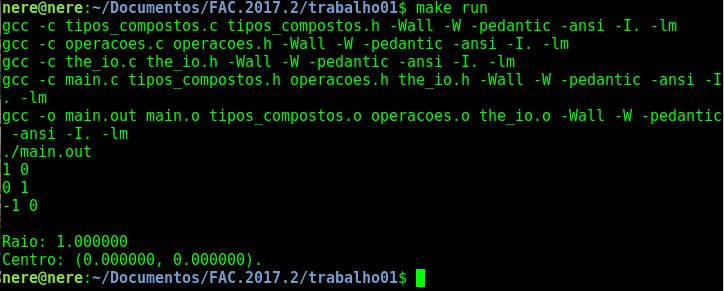
\includegraphics[scale=0.5]{img1.png}
		\end{figure}
		 \paragraph{}	Caso os pontos sejam coolineares, o sistema retorna a seguinte resposta:
		 \begin{figure}[H]
        	\centering
			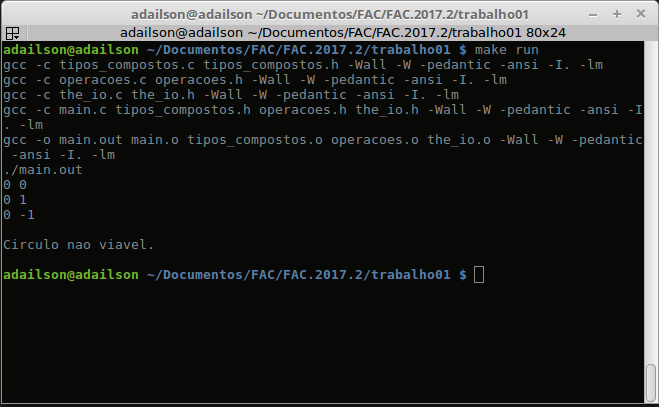
\includegraphics[scale=0.5]{img3.png}
		\end{figure}
\section{Quest\~ao 02}
    \subsection{Racioc\'inio l\'ogico}
        \paragraph{}    A quest\~ao de n\'umero 2 solicita que fosse criado um programa na linguagem C, que ao ser executado informasse a quantidade de par\^ametros enviados no terminal. A exibi\c{c}\~ao dos par\^ametros deve ser numerada pela posi\c{c}\~ao da vari\'avel. Esses par\^ametros s\~ao obtidos pelos argumentos argc e argv injetadas na main. Argc informa a quantidade de par\^ametros inseridos e argv cont\'em um vetor de string com os par\^ametros.
	\subsection{Instru\c{c}\~ao de uso}
        \paragraph{}    Primeiramente, o usu\'ario deve entrar na pasta que cont\'em todos os arquivos do projeto, ap\'os isso, digitar o comando "gcc -o gmp.out give\_me\_parameters.c" e executar o programa com os par\^ametros que desejar na frente. Ex: "./gmp param1 param2 param3"
        
\begin{figure}[H]
	\centering
	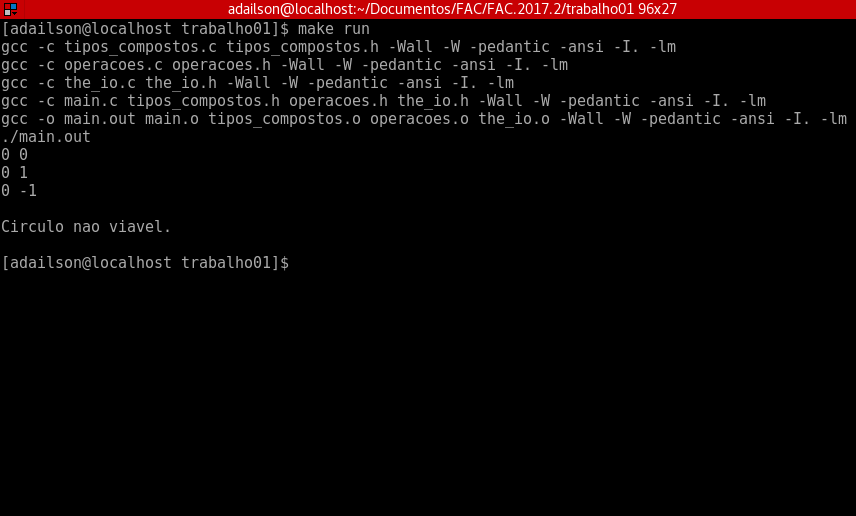
\includegraphics[scale=0.5]{img2.png}
\end{figure}

\end{document}